% =====================================================================
%  Engineering What an Optical Sensor Cannot See  --  Optica Research Article
%  ROUND63 / Certified-Blindness / Three-Ledger line.
%  Binding spec: docs/ROUND63_GPT_ROUND45_RULING_RAW.md Part C (FROZEN by TLSG_PASS).
%  Every numerical claim traces to paper2_optica/CLAIM_SOURCE_MATRIX.md.
%  American spelling.  Companion Letter cited as [COMPANION].
%
%  TODO (final port): opticajnl.cls is NOT installed in this TeX Live toolchain
%  (kpsewhich opticajnl.cls -> empty).  This file is a clean two-column
%  article-class scaffold with Optica-matching typography (full-width title/abstract,
%  numbered sections, spanning figures).  The final submission is a MECHANICAL
%  class swap to \documentclass[10pt,twocolumn]{opticajnl} + \journal{opticajnl}
%  + \setboolean{shortarticle}{false}; no body edits are required.  Logged in
%  BUILD_STATUS.md (Phase 2, class-file status).
% =====================================================================
\documentclass[10pt,twocolumn]{article}

\usepackage[letterpaper,hmargin=0.8in,vmargin=0.9in,columnsep=0.28in]{geometry}
\usepackage{graphicx}
\usepackage{amsmath}
\usepackage{amssymb}
\usepackage{amsthm}
\usepackage{bm}
\usepackage{booktabs}
\usepackage[hidelinks]{hyperref}
\graphicspath{{figures/}}

% --- Optica-like typography ---
\usepackage{times}
\renewcommand{\familydefault}{\rmdefault}
\setlength{\parindent}{1em}
\usepackage[font=footnotesize,labelfont=bf,labelsep=period]{caption}

% --- theorem environments ---
\theoremstyle{plain}
\newtheorem{theorem}{Theorem}
\newtheorem{corollary}{Corollary}
\theoremstyle{definition}
\newtheorem{remark}{Remark}

% --- macros (shared with the companion Letter) ---
\newcommand{\Treq}{T_{\mathrm{req}}}
\newcommand{\Cstar}{C_{\ast}}
\newcommand{\tr}{\operatorname{tr}}
\newcommand{\rank}{\operatorname{rank}}
\newcommand{\eps}{\varepsilon}
\newcommand{\bd}{\beta}
\newcommand{\Lop}{L}
\newcommand{\Bmet}{B}

\title{\vspace{-2.5em}\bfseries\LARGE Engineering What an Optical Sensor Cannot See}
\date{\today}

\begin{document}

% ---------------------------------------------------------------------
% Full-width title + abstract (Optica research-article front matter).
% article twocolumn: use @twocolumnfalse so title/abstract span both columns.
% ---------------------------------------------------------------------
\twocolumn[
  \begin{@twocolumnfalse}
    \vspace{4pt}
    \begin{center}
      {\LARGE\bfseries Engineering What an Optical Sensor Cannot See\par}
      \vspace{10pt}
      {\large [AUTHORS]\par}
      \vspace{3pt}
      {\itshape [AFFILIATION]\par}
      \vspace{2pt}
      {\small\today\par}
    \end{center}
    \vspace{6pt}
    \begin{center}
    \begin{minipage}{0.92\textwidth}
      \noindent\small\textbf{Abstract.} A symmetry of an optical measurement law
      makes a scene subspace exactly invisible. We turn that blindness into a
      calibrated, certifiable design variable. A statistical Noether theorem
      identifies each exact wall with a score-null orbit; a blindness-capacity
      theorem, $\bd_d=\sigma_d$, makes the largest guaranteed-invisible code space
      a measured singular spectrum; a three-ledger theorem separates what finite
      data can certify into a $1:\sqrt{p}:p$ ladder for known, blind, and estimated
      change; and a jet-transmutation corollary shows an exact wall or projection
      restores the higher-amplitude law. A scaling gate and a wave-optics twin
      validate the program. This opens calibrated, publishable optical blindness.
      \par\vspace{6pt}
      \noindent\footnotesize\textcopyright\ 2026. Companion Letter, Ref.~{[COMPANION]}.
    \end{minipage}
    \end{center}
    \vspace{14pt}
  \end{@twocolumnfalse}
]

% =====================================================================
\section{Introduction}
% =====================================================================
A strongly scattering or bandlimited optical channel is usually described by what
it destroys. The received wisdom is that a lost coordinate is simply lost. The
companion Letter~\cite{COMPANION} already separates two invariants that this view
conflates: reconstruction rank, which can collapse to one, and local change
observability, which can stay complete because the first nonzero nuisance-profiled
statistical jet fixes the price of observing each direction. That Letter owns the
Rank--Jet Separation theorem and the algebraic mean wall of a scrambling channel.

Here we take the complementary and constructive step. Rather than accept an
optical sensor's blindness as a defect, we ask what it \emph{cannot} see, whether
that ignorance can be measured, engineered, and certified, and what finite data
then permit us to conclude. The result is a hierarchy of three theorems and one
corollary that turns invisibility into a metrological primitive:

\begin{enumerate}\itemsep2pt
\item exact measurement symmetries create \emph{walls}---score-null orbits on
which no estimator, exposure count, or reconstruction prior can respond
(Section~\ref{sec:walls});
\item calibration measures a wall's \emph{blindness capacity}---the largest code
subspace guaranteed below a declared leak---as a singular spectrum, with a finite
metrological envelope and an explicit noncomposability law (Section~\ref{sec:capacity});
\item geometry and projection \emph{select the jet order}, restoring the desired
higher-amplitude channel through three physically distinct routes
(Section~\ref{sec:jet});
\item unknown tangent dimension imposes a separate $1:\sqrt{p}:p$
\emph{certifiability ladder} on known, blind, and estimated change
(Section~\ref{sec:certify}).
\end{enumerate}

The abstract ingredients---gauge nulls, singular-value min--max, and local
asymptotic normality---are individually classical~\cite{Vaart,DiakonikolasKane};
the contribution is their synthesis into a physical optical metrology program with
a measured dimension--leak curve, a certified cannot-see guarantee, and a
wave-optics transfer chain (Section~\ref{sec:transfer}). The five sections are
organized by theorem, not by chronology; the seventeen-test verification battery,
the honest negatives, and the full proofs are in the Supplement. Every quoted
number traces to a single committed artifact.

% =====================================================================
\section{Symmetry walls of an optical measurement}\label{sec:walls}
% =====================================================================
\begin{figure*}[t]
\centering
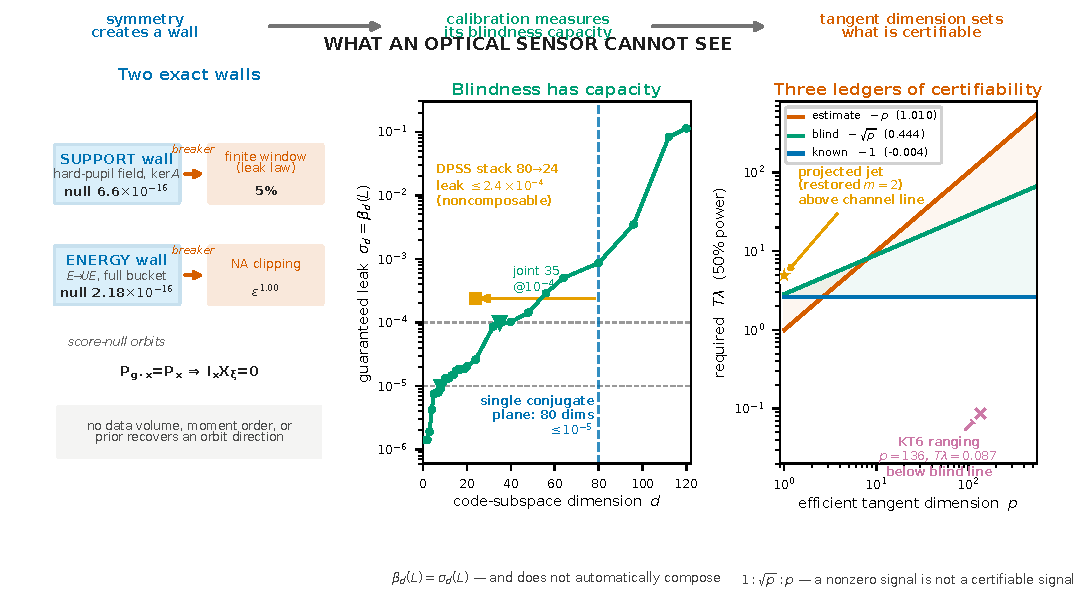
\includegraphics[width=\textwidth]{fig1_hero.pdf}
\caption{\textbf{What the sensor cannot see.} A left-to-right causal spine over
three quantitative panels. \emph{Left --- symmetry walls:} two exact score-null
orbits, the hard-pupil support (field) wall at a maximum leak beyond $2kR$ of
$6.6\times10^{-16}$ and the lossless full-aperture energy (unitary) wall at
$2.18\times10^{-16}$ (both machine zero), each with its one controlled breaker
(finite-window leak law; $\eps^1$ NA clipping). \emph{Center --- blindness
capacity:} the generalized leak singular value $\sigma_d$ versus code-subspace
dimension $d$ (single deterministic joint spectrum), with the single-plane point
($80$ dimensions $\le10^{-5}$ at the fixed conjugate plane), the joint spectrum
point ($35$ dimensions $\le10^{-4}$ over four $z_1$ planes), and the hardware DPSS
route ($\le2.4\times10^{-4}$, whose single-plane SVD capacity does not compose,
$80\!\to\!24$). \emph{Right --- certifiability ladder:} the required
$T\lambda\sim 1:\sqrt{p}:p$ thresholds for known, blind, and estimated change,
with the TLSG-measured $p$-exponents $-0.004/0.444/1.010$; the near-contact KT6
operating point sits below the blind line, and the projected $m=2$ jet sits above
its known-direction channel line. All values are committed frozen artifacts
(KT1~\texttt{@19338a4}, IT1~\texttt{@f13a323}, IT4b~\texttt{@5666d1e},
IT5~\texttt{@c8a0487}, KT6~\texttt{@635ff05}, TLSG~\texttt{@35d858e}).}
\label{fig:hero}
\end{figure*}

Let a scene $x$ lie on a smooth parameter manifold, let the complete observed
record have a dominated law $P_x$ with density $p(y\mid x)$, and let a Lie group
$G$ act on the scene with infinitesimal generator $X_\xi$ for a Lie-algebra
element $\xi$.

\begin{theorem}[Statistical Noether wall]\label{thm:noether}
If the measurement law is $G$-invariant, $P_{g\cdot x}=P_x$ for every $g\in G$,
then every orbit tangent is an exact score-null direction,
\begin{equation}
D_x\log p(Y\mid x)[X_\xi(x)]=0\ \text{a.s.},\qquad I_x\,X_\xi(x)=0,
\label{eq:scorenull}
\end{equation}
so every $f$-divergence, Chernoff distance, and quotient information jet between two
points of one orbit vanishes: no estimator, moment order, exposure count, or
reconstruction prior can distinguish them. Conversely, a smooth constant-rank
integrable distribution that is score-null on a connected neighborhood has integral
leaves that are local blindness orbits.
\end{theorem}

\begin{proof}[Proof sketch]
Differentiate $\log p(y\mid \exp(t\xi)\cdot x)=\log p(y\mid x)$ at $t=0$ to get
\eqref{eq:scorenull}; the score Gramian gives $I_xX_\xi=0$, and equality of the
complete laws gives zero divergence at every finite orbit displacement. The
converse is Frobenius integrability applied to the score-null distribution. Full
statement and the discrete-degeneracy caveat are in Supplement~S1.
\end{proof}

The honest content of Theorem~\ref{thm:noether} is that a symmetry of the
\emph{wave equation} does not by itself create a wall; a wall appears only when the
\emph{full measurement law} inherits the induced parameter action. Two walls of
distinct physical type realize it exactly.

\paragraph{Support (field) wall.}
For a bandlimited mean operator $A$, every $h\in\ker A$ generates a translation
$x\mapsto x+h$ that leaves the mean-channel law invariant---the additive group of
the unmeasured subspace. A hard Fourier pupil restores this wall to machine
precision: the maximum signed-intensity field leak beyond $2kR$ is
$6.6\times10^{-16}$ across all hard-pupil variants and all defocus $z_1$, and the
ideal periodic-code detector wall is $2.07\times10^{-15}$ for $k>k_p$.

\paragraph{Energy (unitary) wall.}
A lossless full-aperture bucket measures only the Hilbert-space norm
$B(E)=\lVert E\rVert_2^2$, so $B(UE)=B(E)$ for every unitary spatial transformation
$U$. A phase-only object change is one orbit of this wall; the measured null is
$2.18\times10^{-16}$ at every order and for every $(\eps,z_2)$. This is the
diagonal subgroup of a much larger \emph{mode-unitary} wall: the energy bucket is
blind not only to phase screens but to any unitary spatial-mode transformation.

\paragraph{The two controlled breakers.}
Each wall has exactly one designed breaker. NA clipping replaces the identity
collector by a projector $P_{\mathrm{NA}}$; $\lVert P_{\mathrm{NA}}UE\rVert^2$ is
no longer invariant and the energy wall breaks at first order, with clip-bucket
slopes $0.97$--$1.03$ that are monotone in $z_2$. A finite object window breaks the
support wall: the full twin develops a noncompact pedestal with detector leak
beyond $2k_p$ equal to $5.3\times10^{-2}$ (field leak $1.6\times10^{-1}$), so
frequency placement alone gives no wall---an exact detector wall additionally
requires a concentration-grade guard (Section~\ref{sec:transfer}). These two
group actions and their breakers are the first entries of a wall periodic table
for an optical chain (Supplement~S1); a parity-symmetric chain and a
polarization-insensitive bucket supply two further rows.

% =====================================================================
\section{Measuring blindness capacity}\label{sec:capacity}
% =====================================================================
An exact wall is a limiting case. In practice one wants the \emph{largest} code
space on which a sensor is guaranteed not to respond to a declared nuisance, and a
number certifying it. Let a calibrated linear leak operator $\Lop:\mathcal C\to
\mathcal Y$ map a code to its forbidden mean-channel response, with the code norm
whitened by the desired in-band metric, and write its singular values ascending,
$\sigma_1\le\cdots\le\sigma_n$. Define the best worst-case leak of a $d$-dimensional
code subspace,
\begin{equation}
\bd_d(\Lop)=\min_{\dim S=d}\ \max_{c\in S,\ \lVert c\rVert=1}\ \lVert \Lop c\rVert .
\label{eq:betadef}
\end{equation}

\begin{theorem}[Blindness capacity]\label{thm:capacity}
$\bd_d(\Lop)=\sigma_d(\Lop)$, attained by the span of the bottom $d$ right singular
vectors; no other $d$-dimensional code family guarantees a smaller worst-case leak.
For a generalized relative-leak certificate with desired-response metric
$\Bmet^\dagger\Bmet$, $\bd_d=\sqrt{\lambda_d}$ where $\Lop^\dagger\Lop\,v=\lambda\,
\Bmet^\dagger\Bmet\,v$. If a calibration returns $\hat\Lop$ with
$\lVert \Lop-\hat\Lop\rVert_{\mathrm{op}}\le\delta$, the bottom-$d$ subspace of
$\hat\Lop$ obeys the metrological envelope
\begin{equation}
\max_{c\in S_d,\ \lVert c\rVert=1}\lVert \Lop c\rVert\ \le\ \sigma_d(\hat\Lop)+\delta .
\label{eq:robust}
\end{equation}
\end{theorem}

\begin{proof}[Proof sketch]
Equation~\eqref{eq:betadef} is the Courant--Fischer min--max characterization of
$\sigma_d$: the bottom-$d$ subspace attains $\sigma_d$, and any $d$-dimensional
subspace meets the orthogonal complement of the bottom $d-1$ singular vectors, so
it contains a unit vector with leak at least $\sigma_d$. The generalized form is
the same statement for the pencil $(\Lop^\dagger\Lop,\Bmet^\dagger\Bmet)$;
\eqref{eq:robust} is Weyl's inequality. Supplement~S2.
\end{proof}

Theorem~\ref{thm:capacity} makes ``cannot see'' a measured spectrum. At the fixed
relay-conjugate plane, $80$ code dimensions are certified below $10^{-5}$ (and
below $10^{-4}$)---a single-plane blindness-capacity point, not an incidental
code-design success. Enforcing invisibility \emph{jointly} over four defocus
planes $z_1\in\{0,2,5,10\}\,$mm costs capacity: $35$ dimensions remain below
$10^{-4}$ jointly ($8$ below $10^{-5}$), so the single-plane requirement buys $45$
extra dimensions. The full ascending spectrum runs from $\sigma_1=1.43\times10^{-6}$
through $\sigma_{64}=4.99\times10^{-4}$ to $\sigma_{120}=1.13\times10^{-1}$: the
plotted capacity curve of Fig.~\ref{fig:hero}. In the $d=64$ subspace the
worst-direction leak is $4.99\times10^{-4}$, while a random in-subspace code leaks
$1.68\times10^{-4}$ in RMS---threefold below the worst direction and ridge-stable
($d$ at $10^{-4}$ is $35$ across regularizers $0/10^{-8}/10^{-6}$). Certified-blind
codes retain a second sensing channel: the random-to-blind eigenvalue ratio is only
$1.20$ ($\ll3$), yet the operational mean leak is $219\times$ lower
($2.58\times10^{-4}$ versus $5.64\times10^{-2}$).

The envelope \eqref{eq:robust} is what upgrades a numerical null space to a
certified instrument property. On a fresh calibration/test split the simultaneous
$\sigma_{64}(\hat\Lop)+\delta$ envelope has coverage $1.000$
($\sigma_{64}=3.4\times10^{-8}$, $\delta=1.07\times10^{-2}$, worst fresh
bottom-$64$ leak $1.99\times10^{-6}$, six orders below the envelope), and at least
$64$ conjugate-plane dimensions stay certified below $10^{-4}$ on fresh
physical-law draws, with a measured minimum of $80$.

% =====================================================================
\section{Restoring the desired jet}\label{sec:jet}
% =====================================================================
\begin{figure*}[t]
\centering
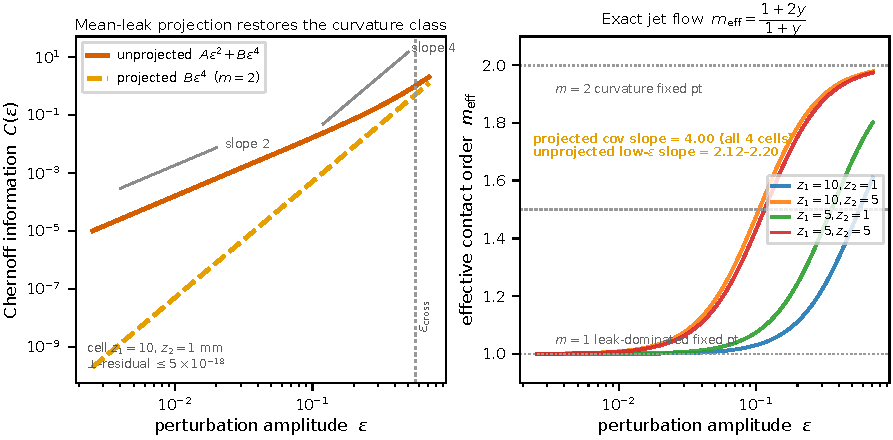
\includegraphics[width=\textwidth]{fig2_jet_transmutation.pdf}
\caption{\textbf{Jet transmutation.} \emph{Left:} the profiled covariance
distance $C(\eps)=A\eps^2+B\eps^4$ reconstructed from the committed fitted
coefficients of the four KT2 cells. Unprojected, a first-order mean leak
($A>0$) gives slope $2$ ($m=1$) at small amplitude; projecting the measured
mean-leak tangent zeroes $A$ and leaves slope $4$ ($m=2$) everywhere, with the
crossover at $\eps_{\mathrm{cross}}=\sqrt{A/B}$. \emph{Right:} the exact logistic
jet flow $\mathrm{d}m_{\mathrm{eff}}/\mathrm{d}\log\eps=2(m_{\mathrm{eff}}-1)
(2-m_{\mathrm{eff}})$ between the integer fixed points $1$ and $2$; the four
measured projected slopes are $4.00$ and the unprojected low-amplitude slopes are
$2.12$--$2.20$. Cross-anchor: the companion integer contact orders $2.038/4.000$
(Ref.~[COMPANION]). Source: KT2~\texttt{@05f1029}.}
\label{fig:jet}
\end{figure*}

The exact walls of Section~\ref{sec:walls} are the endpoints of a continuous
mechanism. Let the profiled Chernoff distance carry two leading operators,
$C(\eps,g)=A\,g^{2a_1}\eps^{2m_1}+B\,g^{2a_2}\eps^{2m_2}$ with $0<m_1<m_2$, and set
$y=(B/A)g^{2(a_2-a_1)}\eps^{2(m_2-m_1)}$. The effective amplitude order
$m_{\mathrm{eff}}=\tfrac12\,\mathrm{d}\log C/\mathrm{d}\log\eps=(m_1+m_2y)/(1+y)$
obeys the exact flow
\begin{equation}
\frac{\mathrm{d}m_{\mathrm{eff}}}{\mathrm{d}\log\eps}
 = 2\,(m_{\mathrm{eff}}-m_1)(m_2-m_{\mathrm{eff}}),
\label{eq:jetflow}
\end{equation}
with fixed points $m_1$ and $m_2$.

\begin{corollary}[Jet transmutation]\label{cor:jet}
A lower-order symmetry-breaking channel ($m_1=1$) drives the strict local
observability class to $m_{\mathrm{eff}}\to1$ as $\eps\to0$; setting its
coefficient to zero by an exact wall, a certified code, or a nuisance projection
places the experiment on the higher-order fixed manifold $m_2=2$ without changing
the scene perturbation. In the near-contact optical case $m_1=1,a_1=0,m_2=2,a_2=2$,
so the crossover invariant is $\eps\,z_2^2=\mathrm{const}$, i.e.\ $z_{2,\ast}\propto
\eps^{-1/2}$.
\end{corollary}

Three physically distinct routes realize the corollary, and they are alternatives,
not factors.

\paragraph{Route 1 --- optical projection.}
Projecting out the measured mean-leak tangent restores the covariance-only slope to
$4.00$ in all four cells, against an unprojected leak-dominated slope of
$2.12$--$2.20$; the orthogonality residual is $\sim10^{-18}$. A generic direction,
by contrast, stays sub-quartic (slopes $1.58$--$2.28$).

\paragraph{Route 2 --- code-space projection.}
Projecting the covariance score off the leak/law span drives the nuisance overlaps
to zero (amplitude $0.36\to0$, medium $0.20\to0$) while retaining $86$--$99\%$ of
the target information.

\paragraph{Route 3 --- hardware concentration.}
A discrete prolate spheroidal (DPSS)~\cite{Slepian} render-and-object window holds the
beyond-$2k_p$ witness leak below $2.4\times10^{-4}$ uniformly in $z_1$ (maximum
$2.38\times10^{-4}$), $349\times$ below the no-window value $8.3\times10^{-2}$; a
naive separable Tukey window reaches only $\sim4\times10^{-2}$ (rim-limited).

These routes do not stack. For several leak routes $L_1,\dots,L_k$ the simultaneous
root-sum-square certificate is governed by the stacked Gram operator, so
\begin{equation}
\bd_d^2=\lambda_d^{\uparrow}\!\Big(\textstyle\sum_i w_i^2\,L_i^\dagger L_i\Big),
\label{eq:noncompose}
\end{equation}
which is not multiplicative in the individual certificates. Concretely, the DPSS
hardware route does not compose with the SVD code route: the single-plane certified
dimension drops from $80$ to $24$ at $10^{-4}$, because the window rotates and
reshapes the operator and trades code-space capacity. A second, independent witness
of the same law is the Tukey apodization, whose joint certified dimension drops from
$35$ to $24$ and which is $93\times$ worse at $d=64$ (apodized relative leak
$4.66\times10^{-2}$ versus $4.99\times10^{-4}$; a rim effect). Independent hardware
modifications change the leak operator and its metric and must be recalibrated
jointly.

% =====================================================================
\section{What finite data can certify}\label{sec:certify}
% =====================================================================
A wall says a change is invisible; blindness capacity says how large a subspace is
guaranteed invisible; the jet order says how a visible change scales. A fourth,
independent price is set by finite data and unknown direction. Whiten the null
covariance, profile every admitted nuisance tangent, and let the efficient
covariance displacement be $A_\perp$ in a symmetric tangent space of dimension $p$,
with efficient signal $\lambda=\tfrac12\lVert A_\perp\rVert_F^2$. For $T$
independent banks the aggregate score experiment is locally
$Z_T\approx\mathcal N(\sqrt T\,\theta,I_p)$ with $\lVert\theta\rVert^2=\lambda$.

\begin{theorem}[Three-ledger certifiability]\label{thm:ledger}
Under this nuisance-profiled reduction, the per-task bank budget for fixed
nontrivial power obeys
\begin{equation}
T\lambda\sim
\begin{cases}
1, & \text{known direction (matched score),}\\
\sqrt{p}, & \text{blind existence (unknown direction),}\\
p, & \text{estimate or localize the direction,}
\end{cases}
\label{eq:ledgers}
\end{equation}
a $1:\sqrt{p}:p$ ladder. Composed with a quotient jet
$A_\perp=\kappa\,g^{a}\eps^{m}B$, the known-direction budget is
$T_{\mathrm{known}}\asymp\kappa^{-2}g^{-2a}\eps^{-2m}$, and the blind and estimation
budgets multiply it by $\sqrt p$ and $p$; adaptation changes the prefactor, never
the physical exponent $2m$.
\end{theorem}

\begin{proof}[Proof sketch]
The matched score $u^\top Z_T$ separates the hypotheses at $T\lambda=O(1)$. For the
blind ledger the invariant $\lVert Z_T\rVert^2$ is $\chi^2_p$ versus
$\chi^2_p(T\lambda)$, separated when $T\lambda\gg\sqrt p$; a uniform spherical
mixture gives a matching minimax lower bound, since its $\chi^2$-divergence from the
null scales as $T^2\lambda^2/p$ and vanishes below $T\lambda\sim\sqrt p$. The
efficient estimator $\hat\theta=Z_T/\sqrt T$ has risk $p/T$, matching the
Cram\'er--Rao bound, so relative error is controlled only at $T\lambda\sim p$.
Supplement~S4.
\end{proof}

A dedicated scaling gate (TLSG) confirms the ladder without a repair round. The
fitted $p$-exponents for the known, blind, and estimation tasks are
$-0.004/0.444/1.010$ against the frozen targets $0,\tfrac12,1$. The matched-score
$50\%$-power contours collapse against $T\lambda$ with coefficient of variation
$\mathrm{CV}=0.125$; the blind contours collapse against $T\lambda/\sqrt p$
($\mathrm{CV}=0.124$) and \emph{fail} against $T\lambda$ alone ($\mathrm{CV}=0.628$),
the signature of the $\sqrt p$ adaptation penalty; the estimation risk collapses
against $T\lambda/p$ ($\mathrm{CV}=0.035$, mean risk $\cdot\,T\lambda/p=0.985$,
i.e.\ the Cram\'er--Rao floor $p/T$).

The ladder also predicts a negative for the right reason. The near-contact
channel-ratio operating point (KT6) sits below the optimal blind tier: its blind
detection power is $0.051$ at a false-positive rate of $0.05$ (rising to $0.056$ and
$0.134$ at $10\times$ and $100\times$ exposure), with $p=136$ and $T\lambda=0.0866$.
The oracle law is nonetheless intact---the near-contact ratio $J_{\mathrm{cov}}/
J_{\mathrm{mean}}\propto z_2^4$ with fitted exponents $3.99$--$4.08$---but the blind
signal-to-floor ratio is $5.4\times10^{-3}\ll1$, below the Wishart $M^2/T$
floor~\cite{BBP}, so
the estimator is killed. This is a boundary of the third ledger, not a failure of
apparatus: the projected $m=2$ covariance channel of Section~\ref{sec:jet} (slope
$4.00$) is by contrast a \emph{known}-direction observable, and sits above its
channel line in Fig.~\ref{fig:hero}.

% =====================================================================
\section{Wave-optics transfer and apparatus constraints}\label{sec:transfer}
% =====================================================================
\begin{figure*}[t]
\centering
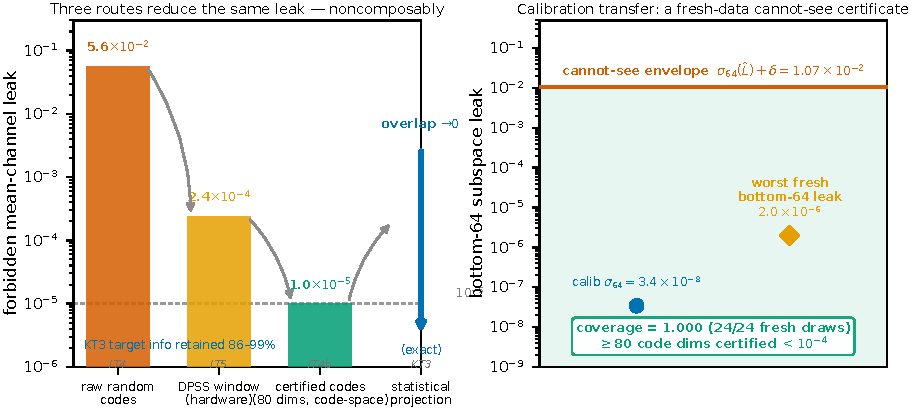
\includegraphics[width=\textwidth]{fig3_routes_transfer.pdf}
\caption{\textbf{Restoration routes and calibration transfer.} \emph{Left:} the
descending leak ladder of the three physically distinct routes plus the exact
statistical projection, all reducing the forbidden mean-channel response---raw
random codes $5.6\times10^{-2}$, DPSS window $2.4\times10^{-4}$, certified codes
$\le10^{-5}$ (single-plane, $80$ dimensions), statistical projection to $0$
(exact)---which are alternatives, not factors. \emph{Right:} calibration transfer
(Eq.~\eqref{eq:robust}) on a fresh calibration/test split: the simultaneous
cannot-see envelope is $1.07\times10^{-2}$, the worst fresh bottom-$64$ leak is
$2.0\times10^{-6}$ (six orders below), coverage is $100\%$ on $24$ fresh draws, and
at least $80$ code dimensions remain certified below $10^{-4}$ at the conjugate
plane. Sources: IT4~\texttt{@33b8ef2}, IT5~\texttt{@c8a0487}, IT4b~\texttt{@5666d1e},
KT3~\texttt{@2430166}, TLSG~\texttt{@35d858e}.}
\label{fig:transfer}
\end{figure*}

The theorems above are algebraic; a bench is not. On the unfiltered
complementary-DMD twin the exact mean wall becomes a reproducible calibrated
residual,
\begin{equation}
L(z_1)=6.94\times10^{-3}+5.92\times10^{-3}\,(z_1/\mathrm{mm})^{0.90},
\label{eq:leaklaw}
\end{equation}
whose floor, coefficient, and exponent are stable across code seeds and code counts
with coefficients of variation $2.2\%$, $2.2\%$, and $0.1\%$. The conjugate-plane
floor is an instrument constant set by fill-factor and macro-pixel staircase
effects (moving $6\%$ and $50\%$ respectively, with $L_{\mathrm{pix}}=7.15\times
10^{-3}$); the pupil does not reduce it. Deterministic beyond-band leak grows with
defocus, from $6.8\times10^{-3}$ at the conjugate plane to $5.4\times10^{-2}$ at
$z_1=10\,$mm and $8.9\times10^{-2}$ at $z_1=20\,$mm; near-conjugate relay imaging
suppresses the propagation term. A full-Maxwell check anchors the model: the
thin-phase-screen speckle contrast $0.467$ agrees with a two-dimensional
finite-element (COMSOL 6.3 Wave Optics, TE) contrast $0.395$ to $15.5\%$. The
covariance signal grows as $\lambda\propto M^{1.8\text{--}1.9}$ in code count
(fitted exponent $1.78$ at mid range, $1.89$ near contact), and the geometry-matched
developed cell extrapolates to $\approx768$ code banks at $2\%$ error for $M=128$,
inside the sealed band $[513,2996]$.

Two apparatus rules follow. First, because a separable Tukey guard reduces the
detector tail only $\sim8$--$40\times$ and never to $10^{-12}$, an exact physical
detector wall requires a concentration-grade (DPSS) guard together with the hard
Fourier pupil---the choice of Section~\ref{sec:jet}, Route~3. Second, binary
rendering must use full-period pulse-width modulation with whole-period bucket
integration: Bayer-ordered spatial dithering doubles the conjugate-plane leak, from
$7.0\times10^{-3}$ to $1.38\times10^{-2}$, above the $10^{-2}$ tolerance.

% =====================================================================
\section{Discussion}
% =====================================================================
Blindness with a symmetry origin is not a defect to be hidden but a quantity to be
calibrated, engineered, and certified. The four objects are independent: a symmetry
decides whether a change exists in the record, the jet order decides how its signal
scales, the singular spectrum decides how large a code space is guaranteed blind,
and the tangent dimension decides whether that signal can be blindly certified. A
physical sensor can therefore \emph{publish} a calibrated dimension--leak frontier
describing the largest code space on which it is guaranteed not to respond to a
declared nuisance, backed by the metrological envelope~\eqref{eq:robust} rather than
an uncertified numerical null. The closest structural cousins---decoherence-free
subspaces~\cite{ZanardiRasetti,LidarChuangWhaley}, dynamical
decoupling~\cite{ViolaKnillLloyd}, and unobservable subspaces in nonlinear
control~\cite{HermannKrener}---share the kernel idea; the optical novelty is the
hardware-calibrated, task-selective blindness with a measured capacity curve and a
finite-sample certifiability ladder. The program is optics-first by design: without
a bench instrument or a second non-optical physical realization the synthesis
belongs in Optica, and the memory-effect phase diagram~\cite{FengMemory} (which
requires a genuine thickness or stacking axis) is deferred. The same
symmetry-first accounting extends to quantum-limited sensing, where a measurement
symmetry likewise sets what no estimator can resolve~\cite{Tsang}. The honest negatives that bound the
scope---a segmented bucket that breaks the mean wall, and a coincidence veto that
repairs medium false alarms while retaining only $24\%$ of scene power---appear with
the positives in Supplement~S5.

% ---------------------------------------------------------------------
\section*{Back matter}
\paragraph{Funding.}[FUNDING/ACKNOWLEDGMENTS]
\paragraph{Acknowledgments.}[FUNDING/ACKNOWLEDGMENTS]
\paragraph{Disclosures.}The authors declare no conflicts of interest.
\paragraph{Data availability.}The committed frozen artifacts underlying every
numerical claim, the claim--source matrix, and the figure scripts are available at
[URL]. See Supplement~1 for the full verification battery, proofs, and the TLSG
gate table.

% =====================================================================
\begin{thebibliography}{99}

\bibitem{COMPANION}
[AUTHORS], Strong optical disorder erases images but preserves local change
observability, companion Letter (2026).

\bibitem{FengMemory}
S.~Feng, C.~Kane, P.~A. Lee, and A.~D. Stone,
Correlations and fluctuations of coherent wave transmission through disordered
media, Phys. Rev. Lett. \textbf{61}, 834 (1988).

\bibitem{ZanardiRasetti}
P.~Zanardi and M.~Rasetti,
Noiseless quantum codes, Phys. Rev. Lett. \textbf{79}, 3306 (1997).

\bibitem{LidarChuangWhaley}
D.~A. Lidar, I.~L. Chuang, and K.~B. Whaley,
Decoherence-free subspaces for quantum computation,
Phys. Rev. Lett. \textbf{81}, 2594 (1998).

\bibitem{ViolaKnillLloyd}
L.~Viola, E.~Knill, and S.~Lloyd,
Dynamical decoupling of open quantum systems,
Phys. Rev. Lett. \textbf{82}, 2417 (1999).

\bibitem{HermannKrener}
R.~Hermann and A.~J. Krener,
Nonlinear controllability and observability,
IEEE Trans. Autom. Control \textbf{22}, 728 (1977).

\bibitem{Vaart}
A.~W. van der Vaart,
\emph{Asymptotic Statistics} (Cambridge University Press, 1998).

\bibitem{DiakonikolasKane}
I.~Diakonikolas and D.~M. Kane,
The sample complexity of robust covariance testing,
Proc. 34th Conf. Learning Theory (COLT), PMLR \textbf{134}, 1511 (2021).

\bibitem{Slepian}
D.~Slepian,
Prolate spheroidal wave functions, Fourier analysis, and uncertainty---V:
the discrete case, Bell Syst. Tech. J. \textbf{57}, 1371 (1978).

\bibitem{BBP}
J.~Baik, G.~Ben Arous, and S.~P\'ech\'e,
Phase transition of the largest eigenvalue for nonnull complex sample covariance
matrices, Ann. Probab. \textbf{33}, 1643 (2005).

\bibitem{Tsang}
M.~Tsang, R.~Nair, and X.-M. Lu,
Quantum theory of superresolution for two incoherent optical point sources,
Phys. Rev. X \textbf{6}, 031033 (2016).

\end{thebibliography}

\end{document}
